\section{Product Perspective}
1)Immagine con shared phenomena

2)This is the UML model of  the whole system, based on a class diagram:
\begin{figure}[H]
    \centering
    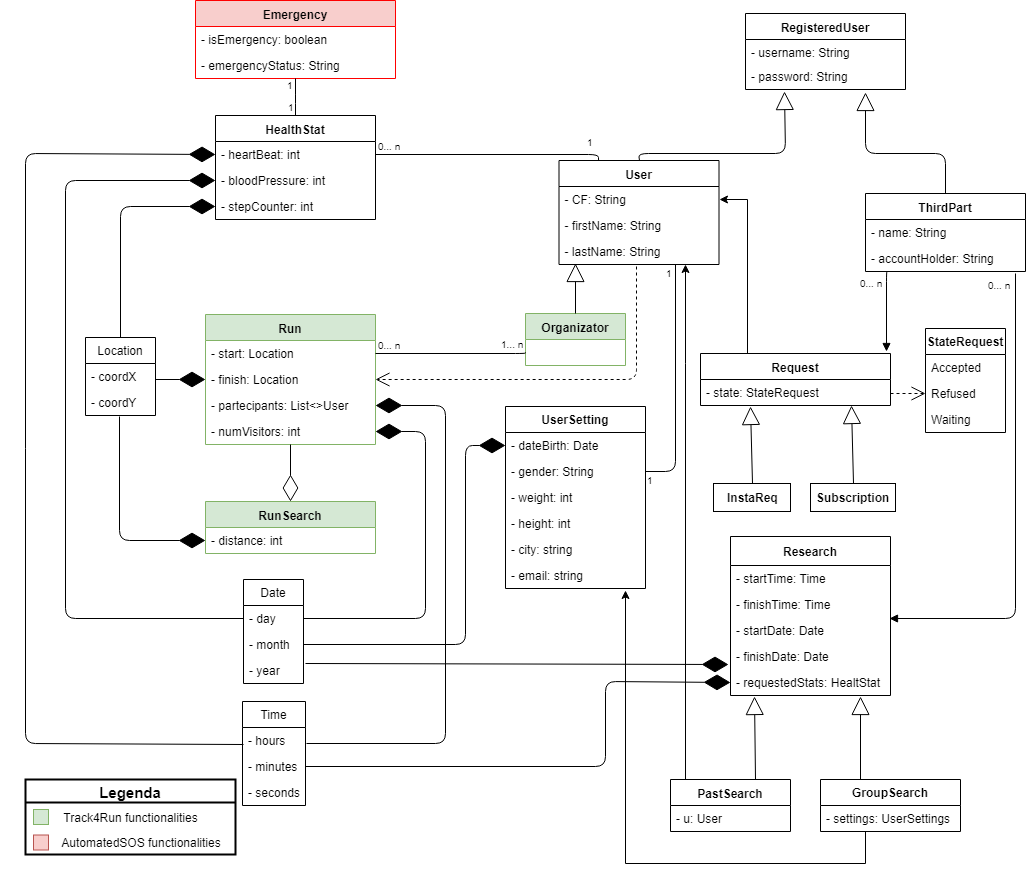
\includegraphics[scale=0.4]{Pictures/UML.png}
  
\end{figure}
3)State charts:

\begin{figure}[H]
    \centering
    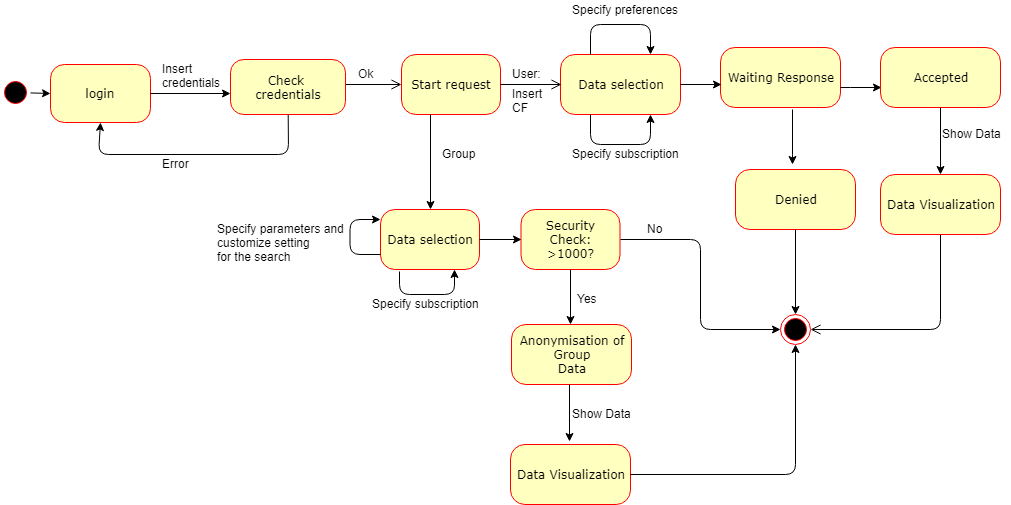
\includegraphics[scale=0.4]{Pictures/state chart 1.png}
    \caption{State chart  \emph{Data4Help} System}
\end{figure}
\newpage
This is a backgroud service that runs in order to keep track of the health status of each user, and notify the SSN in case of Emergency 
\begin{figure}[H]
    \centering
    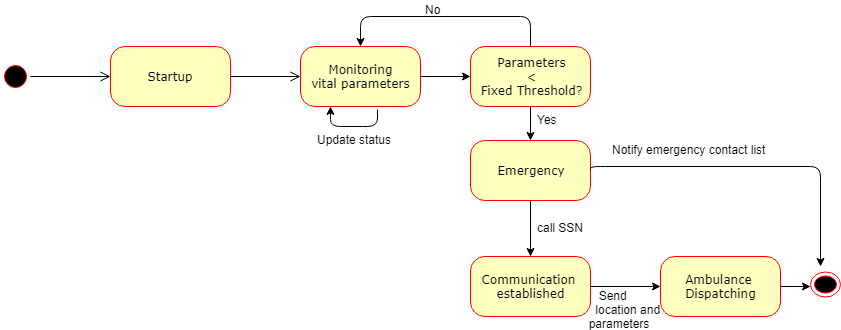
\includegraphics[scale=0.4]{Pictures/state chart 2.png}
    \caption{State chart  \emph{AutomatedSos} System}
\end{figure}
\begin{figure}[H]
    \centering
    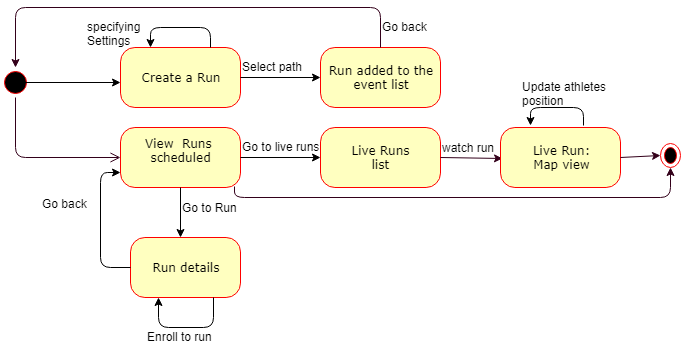
\includegraphics[scale=0.4]{Pictures/statechart3.png}
    \caption{State chart  \emph{Track4Run} System}
\end{figure}